\documentclass[9pt]{beamer}
\usetheme{Warsaw}
\usepackage[utf8]{inputenc}
\usepackage[english]{babel}
\usepackage{amsmath}
\usepackage{amsfonts}
\usepackage{amssymb}
\usepackage{graphicx}
\author{leviathanch | chipforge | foshardware \ (Lanceville Technology)}
\title{Breaking the microchip monopoly}
\setbeamercovered{transparent} 
\setbeamertemplate{navigation symbols}{} 
\logo{lsa.png} 
%\institute{} 
%\date{} 
\subject{A free semiconductor manufacturing standard}
\begin{document}

%\begin{frame}
%\tableofcontents
%\end{frame}

\section[Standard Cells]{}
\begin{frame}{Standard Cells}
\end{frame}

\section[Place'n'Route]{}
\begin{frame}{Open Source Tools}
	\begin{itemize}
        \setlength\itemsep{1em}
		\item graywolf origins in timberwolf
		\item graywolf simulated annealing
		\item graywolf inline syscalls
		\item qrouter purpose and scope
		\item qrouter sequential routing
		\item qrouter formal correctness, esp libresilicon tech
	\end{itemize}
\end{frame}

\begin{frame}{graywolf}
	\begin{itemize}
        \setlength\itemsep{1em}
		\item Originates in Academia: TimberWolf
		\item Simulated annealing
		\item Inline syscalls
	\end{itemize}
\end{frame}

\begin{frame}{Productive Tools}
	\begin{itemize}
        \setlength\itemsep{1em}
		\item Different tool sets like BonnRoute, Cadence, alliance, etc
		\item Similar capabilities with respect to silicon
		\item Just throw man power at large chips - what is automation?
	\end{itemize}
\end{frame}

\begin{frame}{State of the Art}
	\begin{itemize}
        \setlength\itemsep{1em}
		\item Place components for a large chip
		\item Route wires roughly along a chessboard for a large chip
		\item Route detailed tracks and vias for a large chip
		\item Formal correctness: Rip-up and Re-route
		\item Formal style: Sequential/Imperative code
	\end{itemize}
\end{frame}

\begin{frame}{Proposed}
	\begin{itemize}
        \setlength\itemsep{1em}
		\item Decomposition for a large chip
		\item Place components and route for small chips in parallel
		\item Place abstract gates and route recursively
		\item Formal correctness: Reduction from SMT
		\item Formal style: Parallel/Functional code
	\end{itemize}
\end{frame}

\begin{frame}{Divide and Conquer}
	\begin{itemize}
        \setlength\itemsep{2em}
            \item Academia + Industry:
	    \begin{itemize}
            \setlength\itemsep{1em}
		\item Placement and Routing are different problems
		\item All components map to the same problem
	    \end{itemize}
            \item LibreSilicon:
	    \begin{itemize}
            \setlength\itemsep{1em}
		\item Placement and Routing are the same problem
		\item Different components map to different problems
	    \end{itemize}
	\end{itemize}
\end{frame}

\begin{frame}{Parallelism}
	\begin{itemize}
        \setlength\itemsep{1em}
		\item QRouter: None 
		\item BonnRoute: Concurrency + Shared memory model
		\item LSC: map + reduce
	\end{itemize}
\end{frame}

\begin{frame}{Subcell hierarchies}
	\begin{itemize}
        \setlength\itemsep{1em}
		\item Explicit subcell hierarchies through high modularization
		\item Implicit subcell hierarchies through exlining
		\item Preserve hierarchy in compiler interfaces
	\end{itemize}
\end{frame}

\begin{frame}{High modularization}
       \begin{figure}
        \centering
        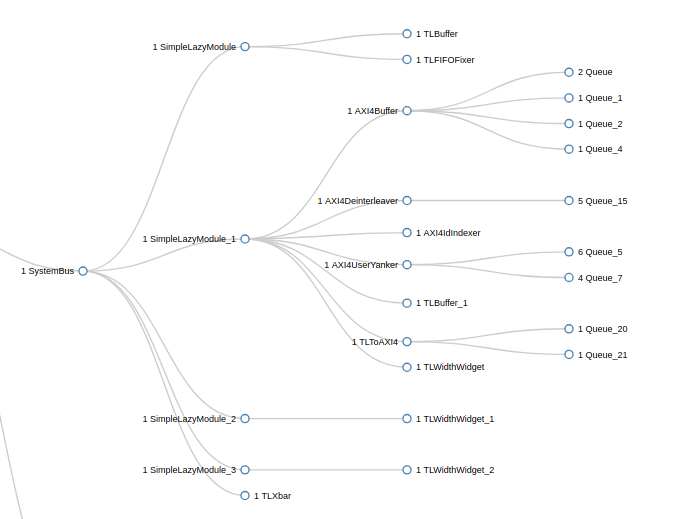
\includegraphics[scale=0.38]{SystemBus.png}
       \end{figure}
\end{frame}

\begin{frame}{Exlining}
	\begin{itemize}
        \setlength\itemsep{1em}
		\item Proof of concept: picorv
	\end{itemize}
\end{frame}


\begin{frame}{SMT2}
	\begin{itemize}
        \setlength\itemsep{1em}
		\item Reduction of a *very* common problem and witty problem to SMT
	\end{itemize}
\end{frame}

\begin{frame}{SMT2}
	\begin{itemize}
        \setlength\itemsep{1em}
		\item Show routing related problem in integer programming
	\end{itemize}
\end{frame}

\end{document}
